\section{Modeling }\label{sec:model}
% 
% {\color{blue} EDITABLE}
% 
% Section outline:
% 
% \begin{enumerate}
% \item \cmark section intro
% \item \cmark fix order from simplest to most complex
% \item Description of DCE and parameter estimation  
% \item\cmark Description of auto ARIMA 
% \item \cmark Description of the two naive methods (random walk and mean), make sure to explain that these methods are naive and simple but not necessarily bad.
% \item\cmark Add a section talking about evaluation methods i.e., MASE, this text is currently written and just sitting at the beginning of the results. 
% 
% \end{enumerate}

In this section, we describe the four different forecasting schema
used in this study, as well as the error metric used to evaluate their
predictive accuracy:
\begin{itemize}
\item The \emph{random-walk} method, which uses the previous value in
  the observed signal as the forecast,

\item The \emph{naive} method, which uses the mean of the
  observed signal as the forecast,

\item The \emph{ARIMA} method, a common linear forecast strategy, and

\item The \emph{LMA} method, which uses a near(est) neighbor forecast
  strategy on a dynamical reconstruction of the signal.
\end{itemize}
ARIMA is based on standard autoregressive techniques.  LMA is designed
to capture and exploit the deterministic structure of a signal from a
nonlinear dynamical system.  The first two methods, somewhat
surprisingly, often outperform sophisticated prediction strategies in
the case of highly complex signals, as discussed below.  

\subsection{Two Simple Prediction Strategies}
\label{sec:simple}

A random-walk predictor simply uses the last observed measurement as
the forecast: that is, the value $p(i)$ at time $i$ is predicted to
be $$p_i = X_{i-1,obs}$$ The \naive ~prediction strategy uses a
rolling average to generate the forecast: the prediction $p_i$ is
simply the average of [[all]] [[no window?  if so, then it's not a
    ``rolling'' average]] observed points up to that point: $$p_i =
\sum_{j=1}^{i-1}\frac{X_{j,obs}}{i-1}$$

While both of these methods are simplistic, they are not without
merit.  For a time series near the high end of the complexity
spectrum---i.e., one that possesses very little predictive
structure---these two methods can actually be the best choice.  In
forecasting currency exchange rates, for instance, sophisticated
econometric techniques and prediction models fail to consistently
outperform the random-walk method~\cite{rwMeese,rwCCE}.  These signals
are volatile, noisy, and possess very little predictive structure, but
they do not---on the average---vary a great deal, so guessing the last
known value is not a bad strategy.  If a signal has a unimodal
distribution with low variance, the \naive ~prediction strategy will
perform quite well---even if the signal is highly complex---simply
because the mean is a good approximation of the future behavior.
Also, a temporal average effects a low-pass filtering operation.  In a
signal with very little predictive structure, then, the \naive
~prediction strategy effectively mitigates the complexity.

Both of these methods have significant weaknesses, however, because
they do not model the temporal patterns of the time series or even the
distribution of its values.  Thus, they cannot track changes in that
structure, which causes them to fail in a number of important
situations.  

Random-walk strategies are a particularly bad choice for time series
that change drastically at every time step.  In the worst case---a
large-amplitude square wave whose period is equivalent to twice the
sample time---a random-walk prediction would be exactly 180 degrees
out of phase with the true continuation.  The \naive ~method would be
better in this situation, since it would always predict the mean.  It
would, however, fail when a signal has a number of long-lived regimes
that have significantly different means.  In this situation, the
inertia of the \naive ~method's rolling mean is a liability and the
random-walk method's nimbleness is an advantage, allowing it to
react quickly to regime shifts.

Of course, a method that could capture and exploit periodic patterns
would be far more effective in these examples.  The LMA method
introduced in Section~\ref{sec:lma} is designed to do exactly that.
[[Couldn't one think about ARIMA as moving in that direction, too?]]
Note, though, that periodic patterns appear only in signals that are
at the low end of the complexity spectrum.  If a signal contains
little predictive structure, forecast strategies like LMA [[and
    ARIMA?]] have nothing to exploit and thus will be beaten out by
the two simple strategies described in this section.  This is explored
further in Sections~\ref{sec:accuracy} and~\ref{sec:results}


\subsection{Linear Forecasting: Seasonal Autoregressive-integrated-moving average(ARIMA){\color{blue} EDITABLE}}\label{sec:arima}
%\begin{enumerate}
%\item\cmark introduce method abstractly and practically, common method basically fitting a hyperplane to data removing seasonality and filtering for noise
%\item\cmark define rigorously, all the backshift operator garbage

%$$\Phi(B^m)\phi(B)(1-B^m)^D(1-B)^dX_i = c + \Theta(B^m)\theta(B)\epsilon_i$$

%$$B^mX_i  = X_{i-m}$$
%\item\cmark discuss that this method needs linear structure to work correctly
%\item \cmark maybe talk about converging to zero and limits on prediction horizon
%\end{enumerate}

%For this \cite{davislinearts}

When there is evidence a generating process exhibits predictive structure an obvious strategy would be to fit a hyperplane to the dataset and then use this hyperplane to forecast new data points. This is a very old technique stemming back to Yule in 1927\cite{weigend93} with his invention of autoregressive forecasting, which forecasts the next time step through a weighted average of the past $p$ time-steps, i.e., $$p_i = \phi(B)X_{i,obs}.$$ Here $\phi(z)$ is a polynomial of degree $p$ and $B$ is the backshift operator, i.e., $$B^mX_i  = X_{i-m,obs}.$$
To improve this method further--especially in the presence of noisy data---one could allow for some wiggle room by adding a moving average of white noise to the model: $\theta(B)\epsilon_i$, where $\theta(z)$ is a polynomial of degree $q$ and $\{\epsilon_i\}\sim WN(0,\sigma^2)$. Finally if there is evidence of non-stationarity an initial differencing (integrated) is applied as an attempt to remove that non-stationarity: $(1-B^d)X_i$. Combining these three give us a nonseasonal  ARIMA$(p,d,q)$ model:  $$\phi(B)(1-B)^dX_i = \theta(B)\epsilon_i.$$ Where $p$, $d$ and $q$ correspond to the orders of the autoregressive, integrated and moving average models respectively. If periodic structure is present a seasonal ARIMA$(p,d,q)(P,D,Q)_m$ is often used and is defined by:$$\Phi(B^m)\phi(B)(1-B^m)^D(1-B)^dX_i = \Theta(B^m)\theta(B)\epsilon_i.$$ Here $\Phi(z)$ and $\Theta(z)$ are polynomials of degree P and Q respectively, and $m$ is the seasonal frequency. Forecasting is then done in two steps, first the integrated step is performed to remove non-stationarity. $$\hat{X_i} = (1-B^m)^D(1-B)^d X_{i,obs}.$$ Then forecasts are made by evaluating $$\Phi(B^m)\phi(B)\hat{X_i} = \Theta(B^m)\theta(B)\epsilon_i.$$

There is a vast amount of theory and literature on constructing, fitting and forecasting with this class of models. However, this is not the focus of this paper and  we refer the reader to \cite{davislinearts} for an in-depth exploration. In this paper, we intend to explore how predictive accuracy of several different forecasting schema correlates with signal complexity. As such, we use ARIMA$(p,d,q)(P,D,Q)_m$ (or simply ARIMA) models as an out of the box black box linear forecasting scheme. To do this we use an automated fitting and forecasting techniques described in \cite{autoARIMA}. This technique automatically selects model and differencing orders: $p, d, q, P, D, Q$ and $m$ as well as fitting the corresponding polynomials to the time series. Hyndman and Khandakar use unit root tests to select differencing orders, $d$ and $D$. In particular, they use a combination of  
KPSS unit-root tests \cite{KPSSunit} and their own extension of Canova-Hansen test \cite{Canova1995}. To do model order selection they use the Akaike information criterion (AIC) \cite{akaike1974} conditioned on the maximized likelihood of the  model fitted to the differenced data, $(1-B^m)^D(1-B)^d X_{i,obs}$ \cite{autoARIMA}. For more detail on this fitting process see \cite{autoARIMA}.

ARIMA forecasting is a time tested modelling process which uses a global linear fit and adjustments for seasonality, non-stationarity and noise. If a generating process fits into this category then this model is a great short term predictor. If information is instead being transmitted in a nonlinear way this global linear fit falls apart. One other weakness of this method is that if long prediction horizons are needed the forecast is guaranteed to converge to the mean after some number of predictions (dependent on model order). For this reason, we limit all methods to doing multiple 1-step predictions as to not handicap this method. 

\subsection{Nonlinear Forecasting: Lorenz Method of Analogues (LMA){\color{blue} EDITABLE}}\label{sec:lma}

When a generating process exhibits deterministic predictive nonlinear structure a common approach is to reconstruct the generating processes dynamics using a technique called delay-coordinate embedding and then use the geometric structure of this reconstruction as a proxy for the information transmission occurring in the underlying process to predict the future. In this section we discuss the theory and implementation of this forecasting scheme. 


 \subsubsection{Reconstructing hidden dynamics {\color{blue} EDITABLE}}



Delay-coordinate embedding allows one to reconstruct a dynamical system's full
state-space dynamics from a \emph{single} scalar time-series
measurement---provided that some conditions hold regarding that data.
Specifically, if the underlying dynamics and the measurement
function---the mapping from the unknown state vector $\vec{X}$ to the
scalar value $X_{i,obs}$ that one is measuring---are both smooth and generic,
Takens~\cite{takens} formally proves that the delay-coordinate map
\[
F(\tau,m)(\vec{X}) = ([X_{i+\tau,obs} ~ X_{i+\tau,obs} ~ \dots ~X_{i+m\tau,obs}])
\]
from a $d$-dimensional smooth compact manifold $M$ to $\mathbb{R}^{2d+1}$,
where $t$ is time, is a diffeomorphism on $M$---in other words, that
the reconstructed dynamics and the true (hidden) dynamics have the
same topology.

This is an extremely powerful result: among other things, it means
that one can build a formal model of the full system dynamics without
measuring (or even knowing) every one of its state variables.  This is
the foundation of this modeling approach.
The first step in the process is to estimate values for the two free
parameters in the delay-coordinate map: the delay $\tau$ and the
dimension $m$.  We follow standard procedures for this, choosing the
first minimum in the average mutual information as an estimate of
$\tau$ \cite{fraser-swinney} and using the false-near(est) neighbor
method of \cite{KBA92} to estimate $m$.  A
plot of the data from Figures~\ref{fig:col-ts}-\ref{fig:svd-ts-colored}, embedded following this
procedure, are shown in Figure~\ref{fig:embedding}.


 \begin{figure}
   \centering
\begin{subfigure}{\columnwidth}
    \includegraphics[width=\columnwidth]{figs/colipc3d.png}
    \caption{\col }
    \label{fig:colEmbedding}
  \end{subfigure}%  \\
  
    \begin{subfigure}{\columnwidth}
    \includegraphics[width=\columnwidth]{figs/gcc3dipc.png}
    \caption{\gcc}
    \label{fig:gccEmbedding}
  \end{subfigure} 
  \\
  \begin{subfigure}{\columnwidth}
    \includegraphics[width=\columnwidth]{figs/svd53dipc2.png}
    \caption{\svdfive}
    \label{fig:svdfiveEmbedding}
  \end{subfigure}%   
%  
 
   
     %\includegraphics[width=\textwidth]{figs/colipc3d.png}
     \caption{A 3D projection of the delay-coordinate embeddings of the traces
 from: (a) \col seen in Figure~\ref{fig:col-ts} (b)\gcc seen in Figure~\ref{fig:gcc-ts} and (c) \svdfive seen as the fifth regime in Figure~\ref{fig:svd-ts-colored}.
 }
 \label{fig:embedding}
 \end{figure}



%% can cut for space if need be:
The coordinates of each point in these plots are differently delayed
elements of the instructions per cycle time series
$X_{i,obs}$: that is, $X_{i,obs}$ on the first axis, $X_{i+\tau,obs}$ on the second,
$X_{i+2\tau,obs}$ on the third, and so on.
Structure in these kinds of plots---clearly visible in
Figure~\ref{fig:embedding} (a) is an indication of
structure in the information transmission process, that can be leveraged for prediction. Where the water becomes muddy is with embedding like those in Figure~\ref{fig:embedding} (b) \& (c). Figure~\ref{fig:embedding} (b) shows little to no structure, this embedding is essentially a noise cloud; with an embedding like this we would expect the forecast accuracy that uses this structure to be lacking. However, with Figure~\ref{fig:embedding} (c) more structure is present but the structure is surrounded in noise. Is the structure enough to aid in accurately forecasting the signal? This is a difficult question to answer and one that comes back to the main contributions of this paper. It may be that \gcc has some redundancy but that structure is not amenable to this method, similarly \svdfive clearly has structure but it is obfuscated by noise. By quantifying the balance between normalized redundancy (predictive structure) and entropy for these real valued time series, we can begin to answer these questions.  If enough (redundancy) predictive structure is present in these embeddings as seen in Figure~\ref{fig:embedding} (a) and possibly in (c), that structure can be used to build a forecast model which we discuss in the next section.
 \subsubsection{LMA: Using dynamics in forecasting {\color{blue} EDITABLE}}

Given a nonlinear model of a deterministic dynamical system in the
form of a delay-coordinate embedding like those in Figure~\ref{fig:embedding},
one can build deterministic forecast algorithms by capturing and
exploiting the geometry of the embedding.  Many techniques have been
developed by the dynamical systems community for this purpose
(e.g.,~\cite{weigend-book,casdagli-eubank92,Smith199250}).  Perhaps the most straightforward
is the ``Lorenz method of analogues'' (LMA), which is essentially
nearest-neighbor prediction in the embedded state
space~\cite{lorenz-analogues}.  Even this simple algorithm---which
builds predictions by finding the nearest neighbor in the embedded space of the given point, then taking that neighbor's path as the
forecast, provides accurate forecasts when the generating process is a deterministic dynamical system. In particular, when an observation in a time series has redundancy in the form of nonlinear predictive structure this forecast scheme should be a great choice. However, since this method is based on near-neighbor prediction in a reconstructed state-space, if a system does not exhibit deterministic structure this method can do quite poorly. {\color{red}[[Joshua:Not a fan of this wording]]}
%% [[If space: Add a segue sentence: next section uses permutation
%% entropy to explore that conjecture.]]

%\subsection{Comparing Prediction Accuracy}





\subsection{Prediction Accuracy: Mean Absolute Scaled Error (MASE) {\color{blue} EDITABLE}}
\label{sec:accuracy}

In order to analyze correctness of each prediction we split each time series into two pieces: the first 90\% referred to as the ``learning" or ``training" signal, $\{X_{i,obs}\}_{i=1}^{n}$ and the last 10\% known as the ``test" or ``correct" signal $\{c_j\}_{j=n+1}^{k+n+1}$. The learning signal is used to train an initial model (e.g., LMA or ARIMA) as described in Section \ref{sec:model}. The test signal is used both to assess the models forecasting accuracy and for any refitting that may be necessary. In particular, we perform $k$ one-step predictions, after each one-step prediction\footnote{We would like to note that this rebuilding occurs due to a problem with ARIMA models converging to a mean prediction if too long of a prediction horizon is used, this is not a handicap of either LMA or na\"ive.} we append the training signal with the next point in the correct signal $c_j$, refit the model taking into account the new system measurement and perform another prediction. This is repeated $k$ times to obtain $\{p_j\}_{j=n+1}^{k+n+1}$.

As a figure of merit we calculate the Mean Absolute Scaled Error (MASE)\cite{MASE} between the true and predicted signals: 
%In order to compare the resulting forecasts we calculate the Mean Absolute Squared Error (MASE)\cite{MASE} between the true and predicted signals:
$$MASE = \sum_{j=n+1}^{k+n+1}\frac{|c_j-p_j| }{\frac{k}{n-1}\sum^n_{i=2}|X_{i,obs}-X_{i-1,obs}|}$$
The scaling term for MASE:
$$\frac{1}{n-1}\sum^n_{i=2}|X_{i,obs}-X_{i-1,obs}|$$ 
is the average in-sample forecast error for a random walk prediction $(p_i=X_{i-1,obs})$. This error method was introduced in \cite{MASE} as a ``generally applicable measurement of forecast accuracy without the problems seen in the other measurements." We chose MASE because it allows for fair comparison across varying methods, prediction horizons and signal scales. When a forecast results in a $MASE<1$ the prediction method produced, on average, smaller errors than the one-step errors from the in-sample random walk forecast strategy. Analogously, $MASE>1$ means that the prediction method did worse, on average than the one-step errors for the in-sample random walk forecast strategy. 

Table \ref{tab:error} provides the MASE distributions {\color{red}[[Joshua: Ryan, Is this the right word? we give mean $\pm$ std. dev but some have very skewed right tails]]} for each of the eight signals and three prediction strategies, these are averaged over 15 runs of each signal-method combination. For later comparison, Table \ref{tab:error} also has the complexity measure we introduce in Section  \ref{sec:meaComplex}. 



To aid in a conceptual understanding of this error metric we provide example forecasts in Figure~\ref{fig:forecast-example}. In plots like this we plot $(c_j,p_j)$, visually points close to the line $y=x$, i.e. the line $p_j = c_j$ are more accurate. Forecasts which stay close to the line are more accurate than forecasts that stray away from it. 


\begin{figure}[htbp]
  \centering
      \begin{subfigure}{0.33\columnwidth}
    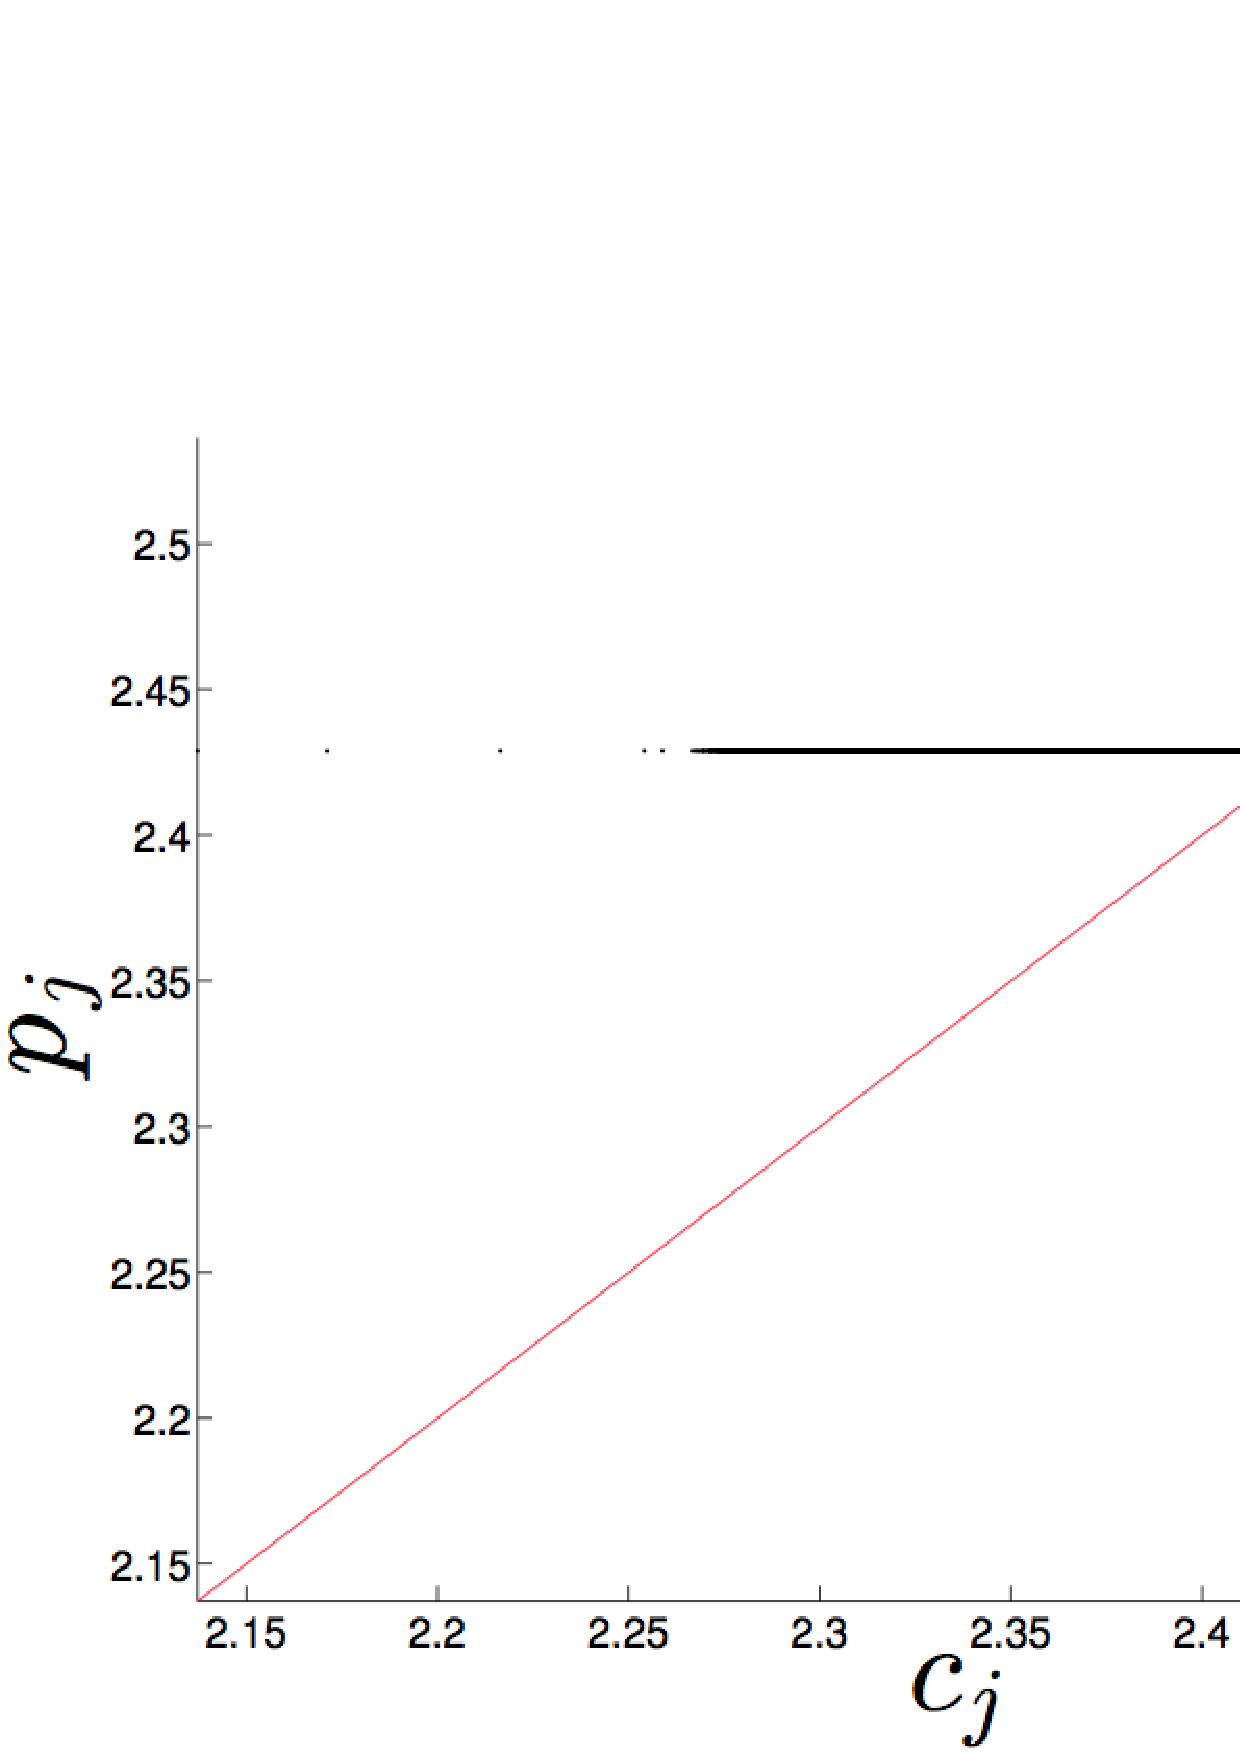
\includegraphics[width=\columnwidth]{figs/colMeanForecast.png}
    \caption{\col\\ na\"ive }
    \label{fig:gccMEAN}
  \end{subfigure}%
   \begin{subfigure}{0.32\columnwidth}
    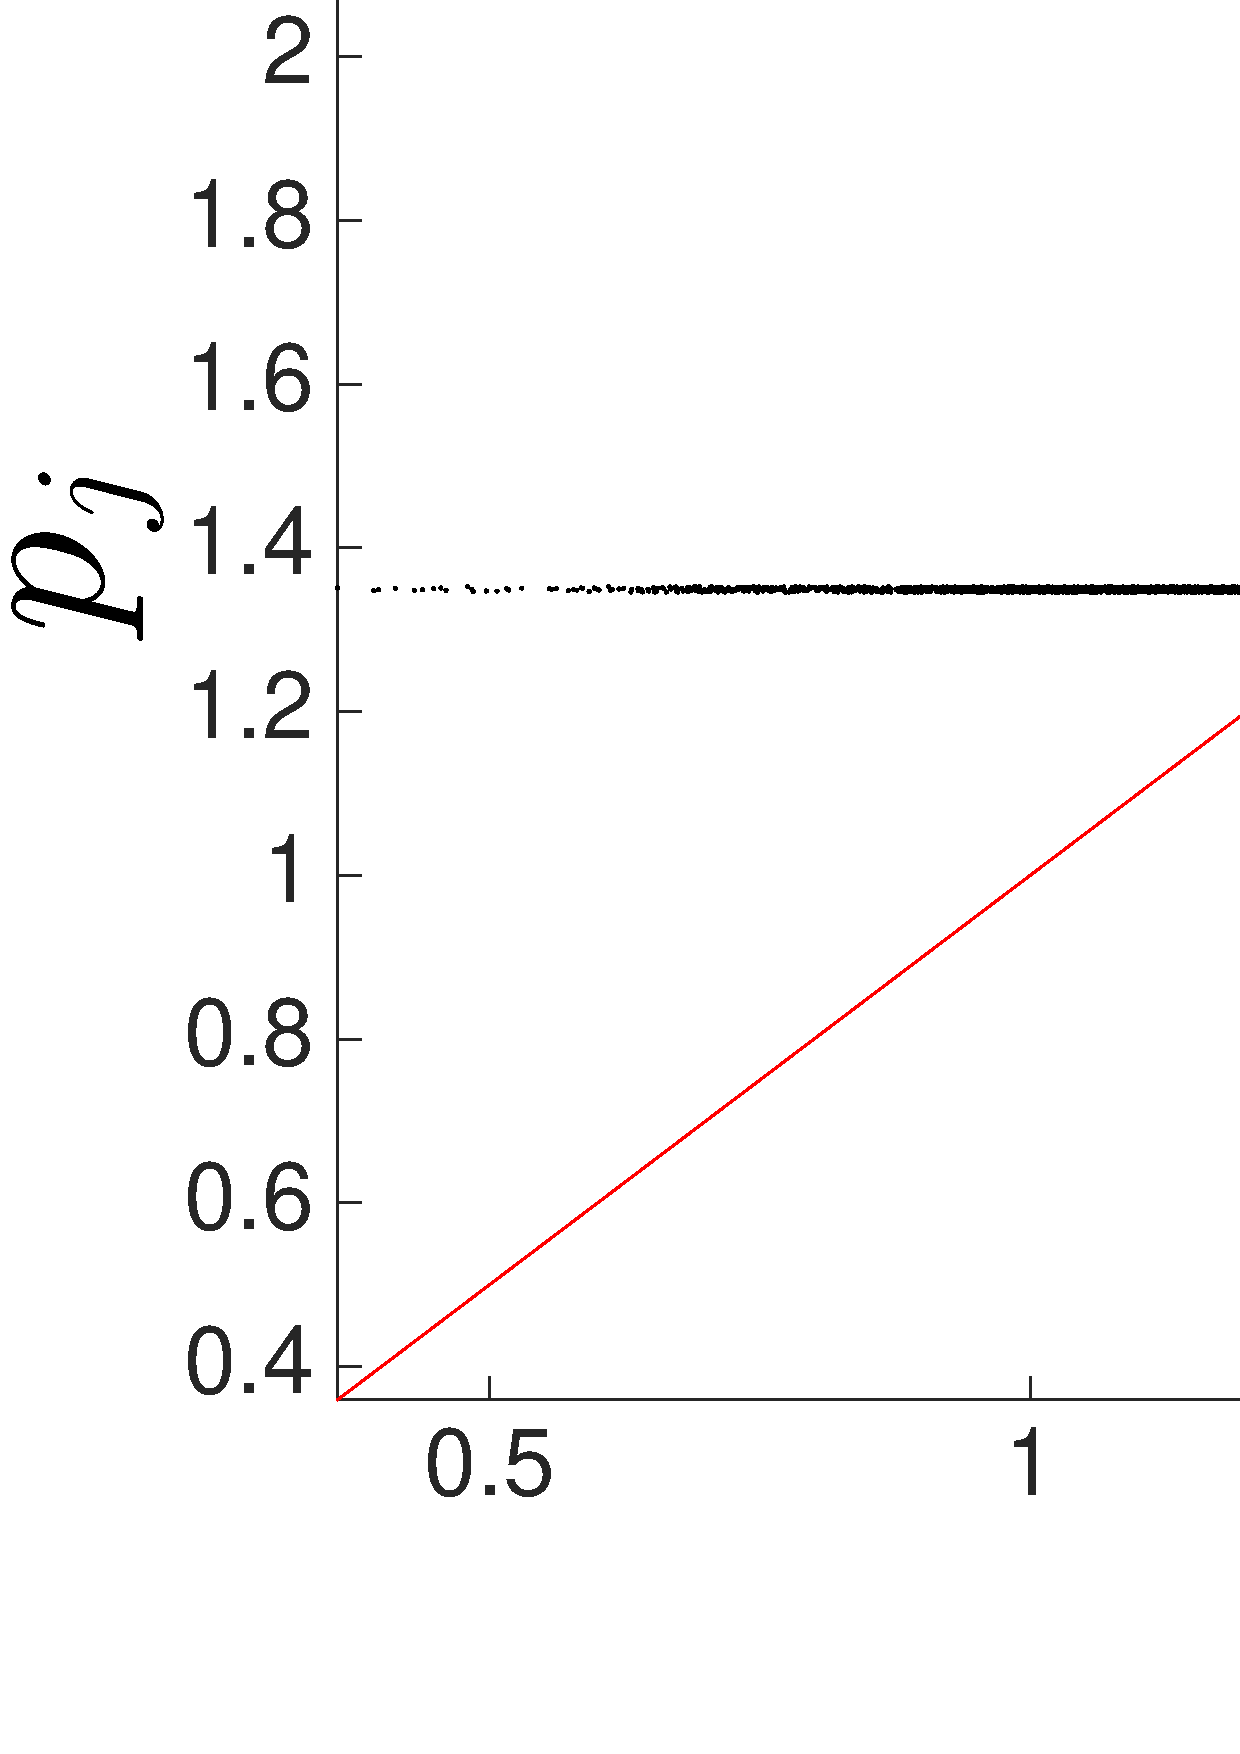
\includegraphics[width=\columnwidth]{figs/gccMeanForecast.png}
    \caption{\gcc\\ na\"ive }
    \label{fig:gccMEAN}
  \end{subfigure}% 
     \begin{subfigure}{0.32\columnwidth}
    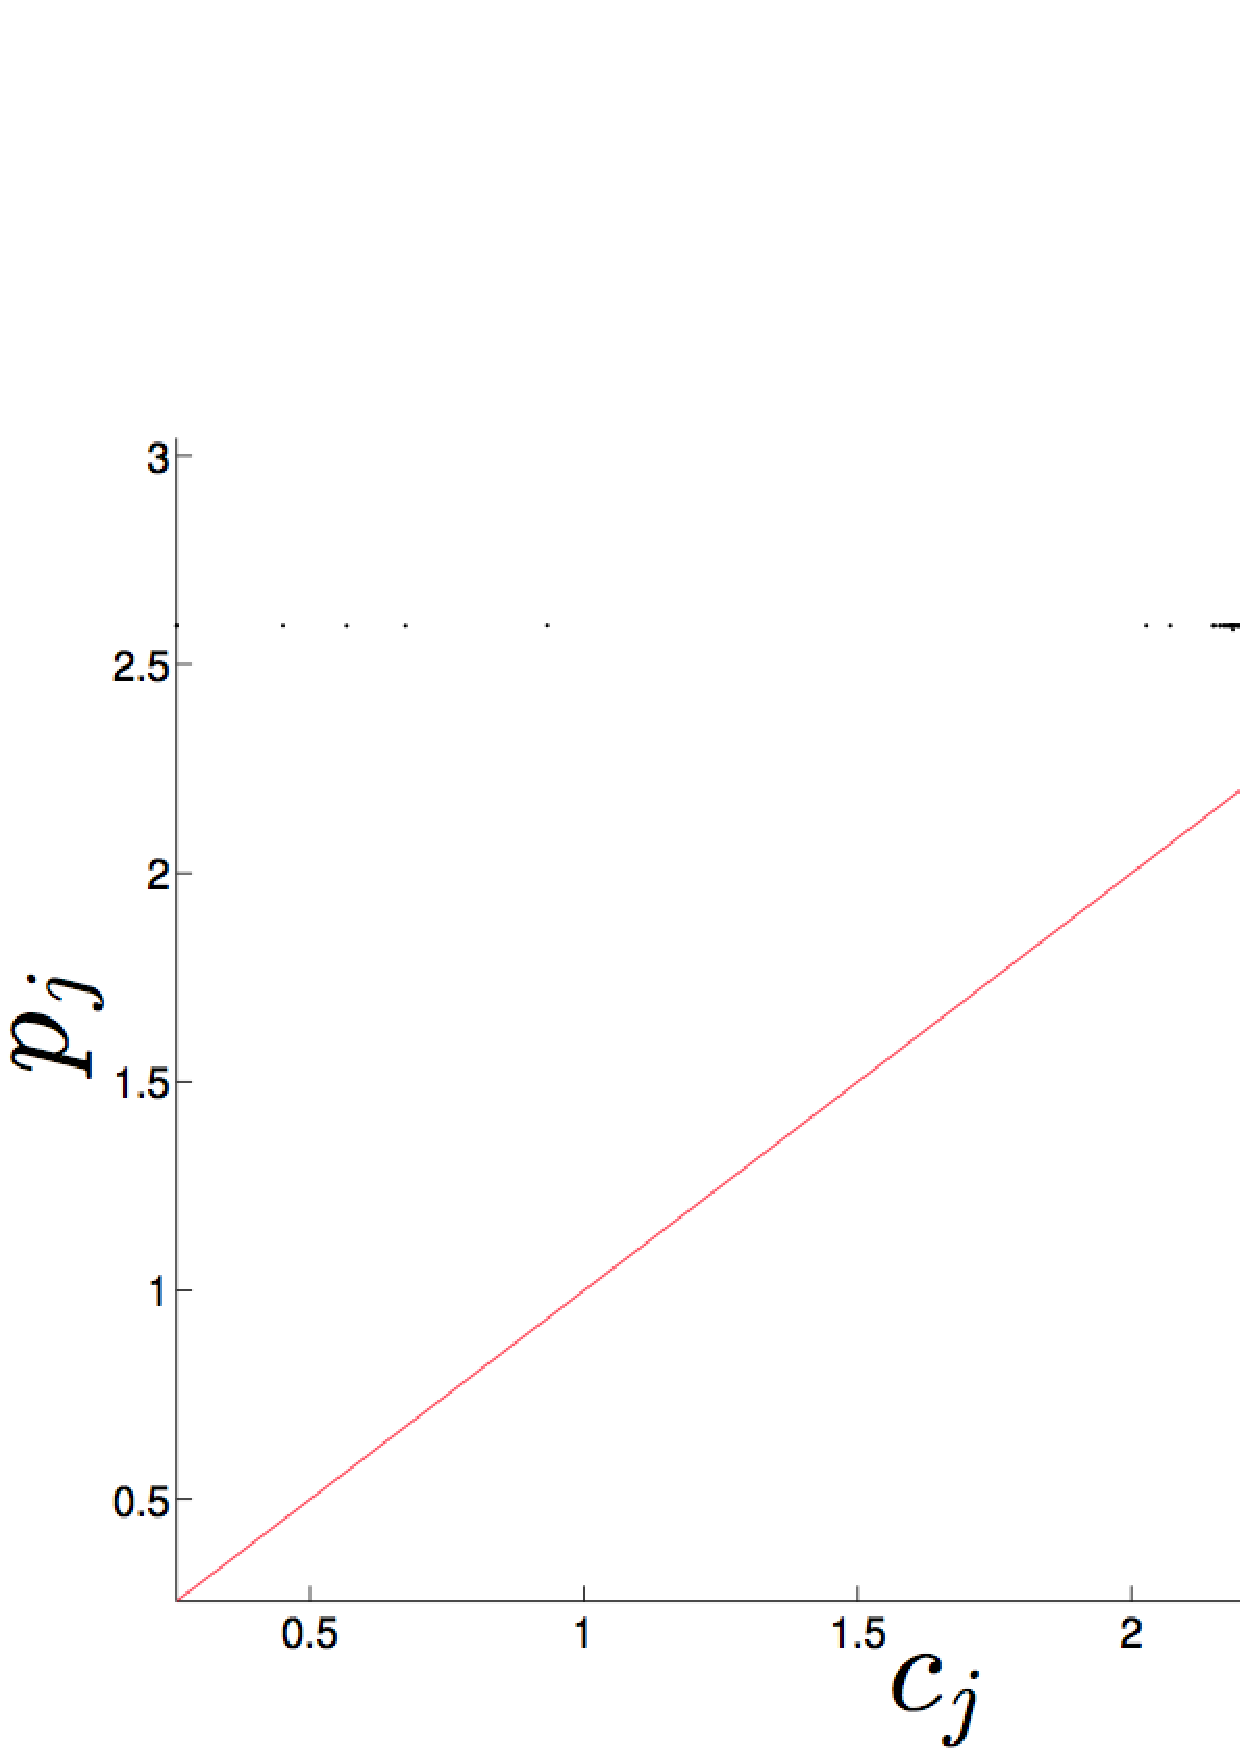
\includegraphics[width=\columnwidth]{figs/svdfiveMeanForecast.png}
    \caption{\svdfive\\ na\"ive }
    \label{fig:gccMEAN}
  \end{subfigure}%      
  \\
    \begin{subfigure}{0.32\columnwidth}
    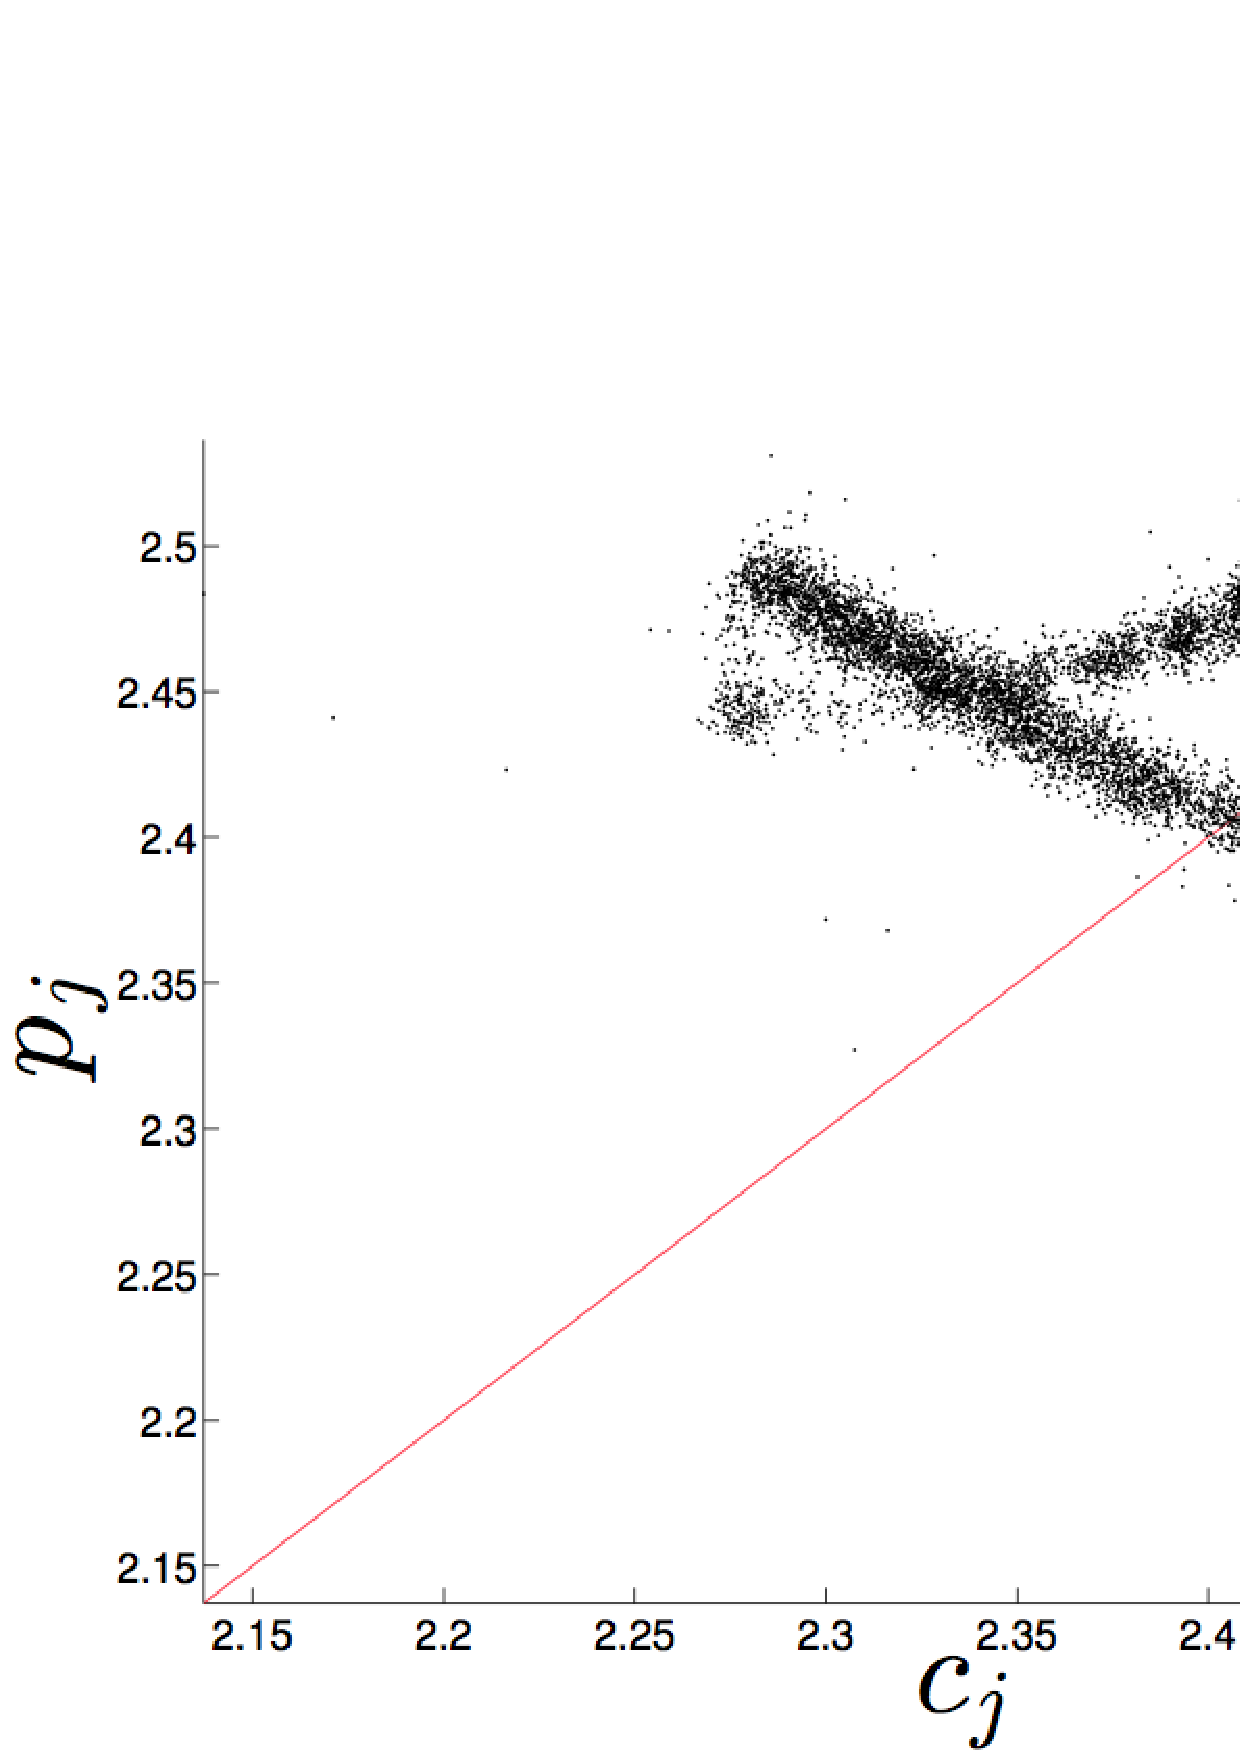
\includegraphics[width=\columnwidth]{figs/colARIMAForecast.png}
    
    
    \caption{\col ARIMA}
    \label{fig:colARIMA}
  \end{subfigure}
  \begin{subfigure}{0.32\columnwidth}
    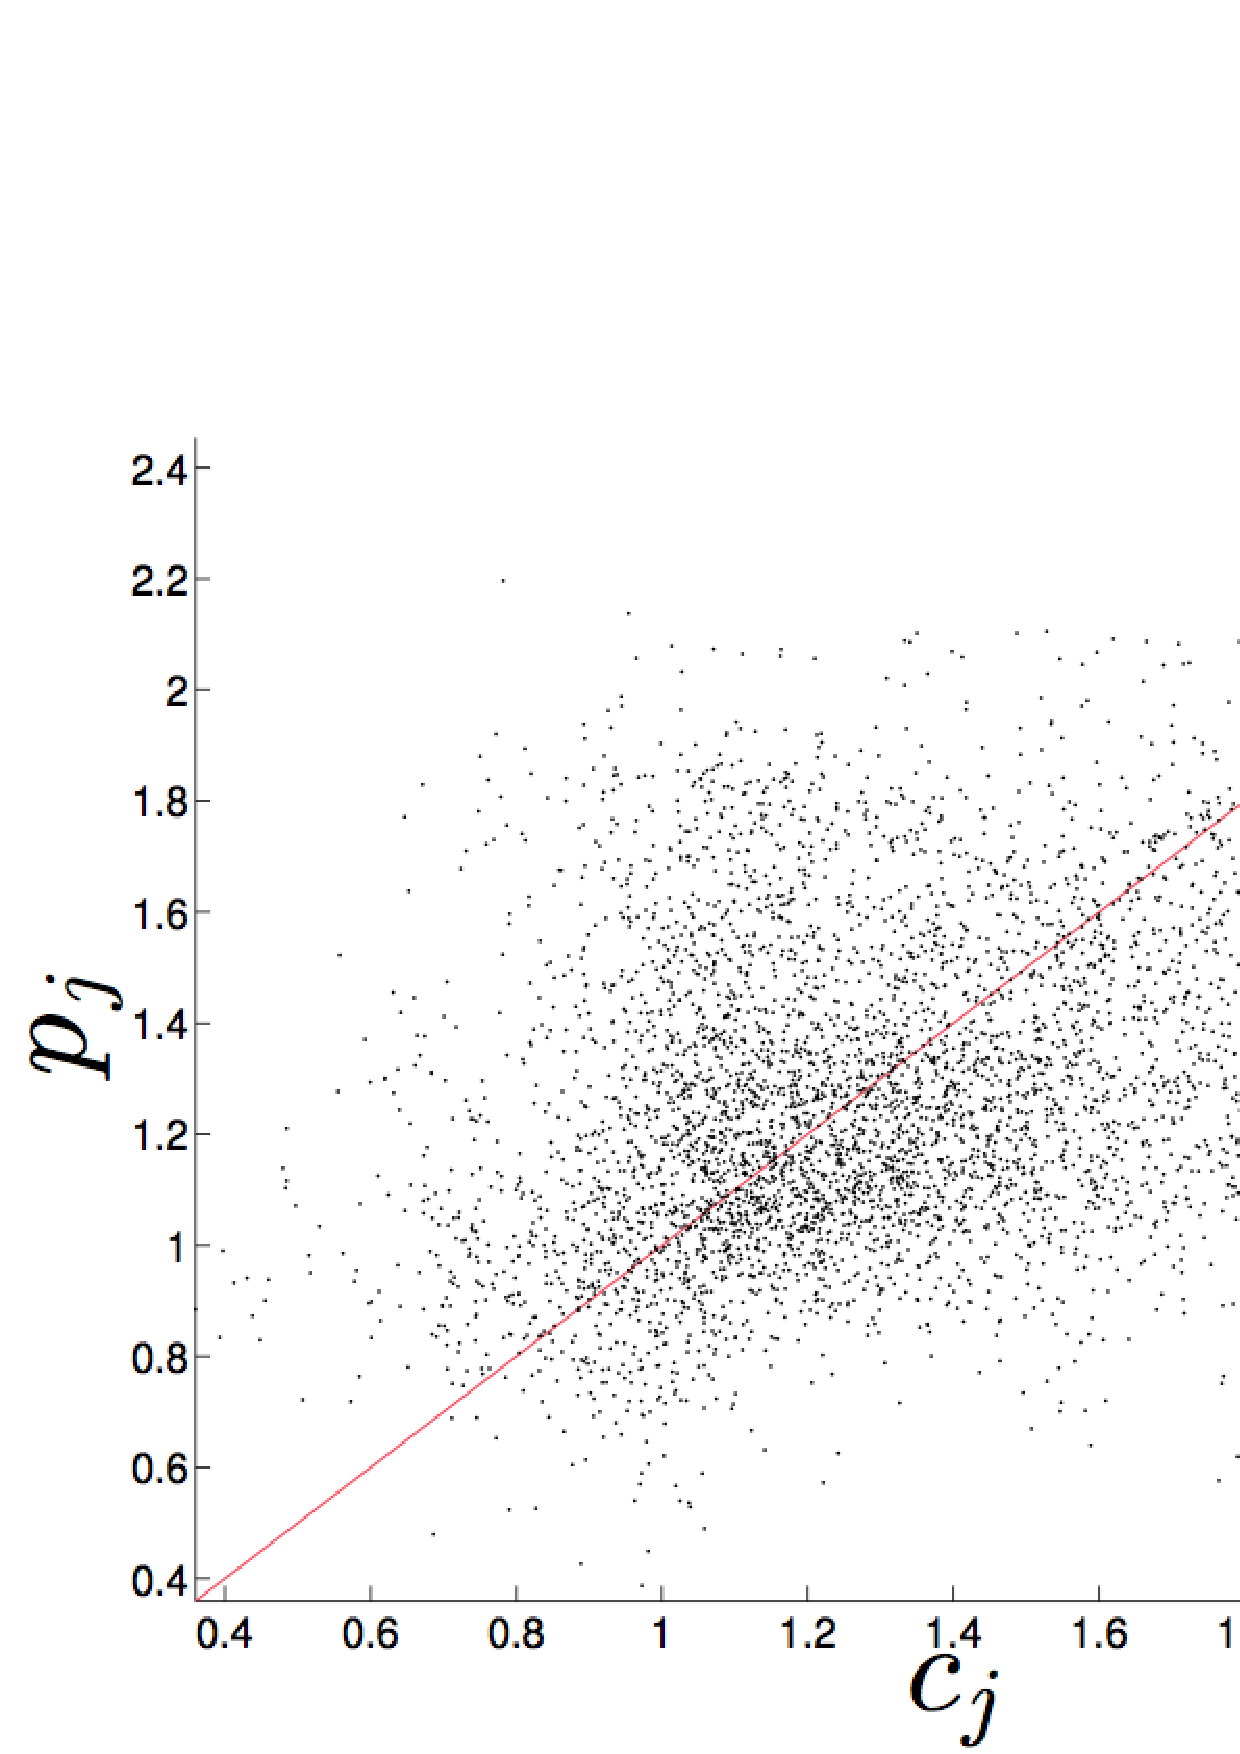
\includegraphics[width=\columnwidth]{figs/gccARIMAForecast.png}
    \caption{\gcc \\ ARIMA }
    \label{fig:gccARIMA}
  \end{subfigure}%
  \begin{subfigure}{0.32\columnwidth}
    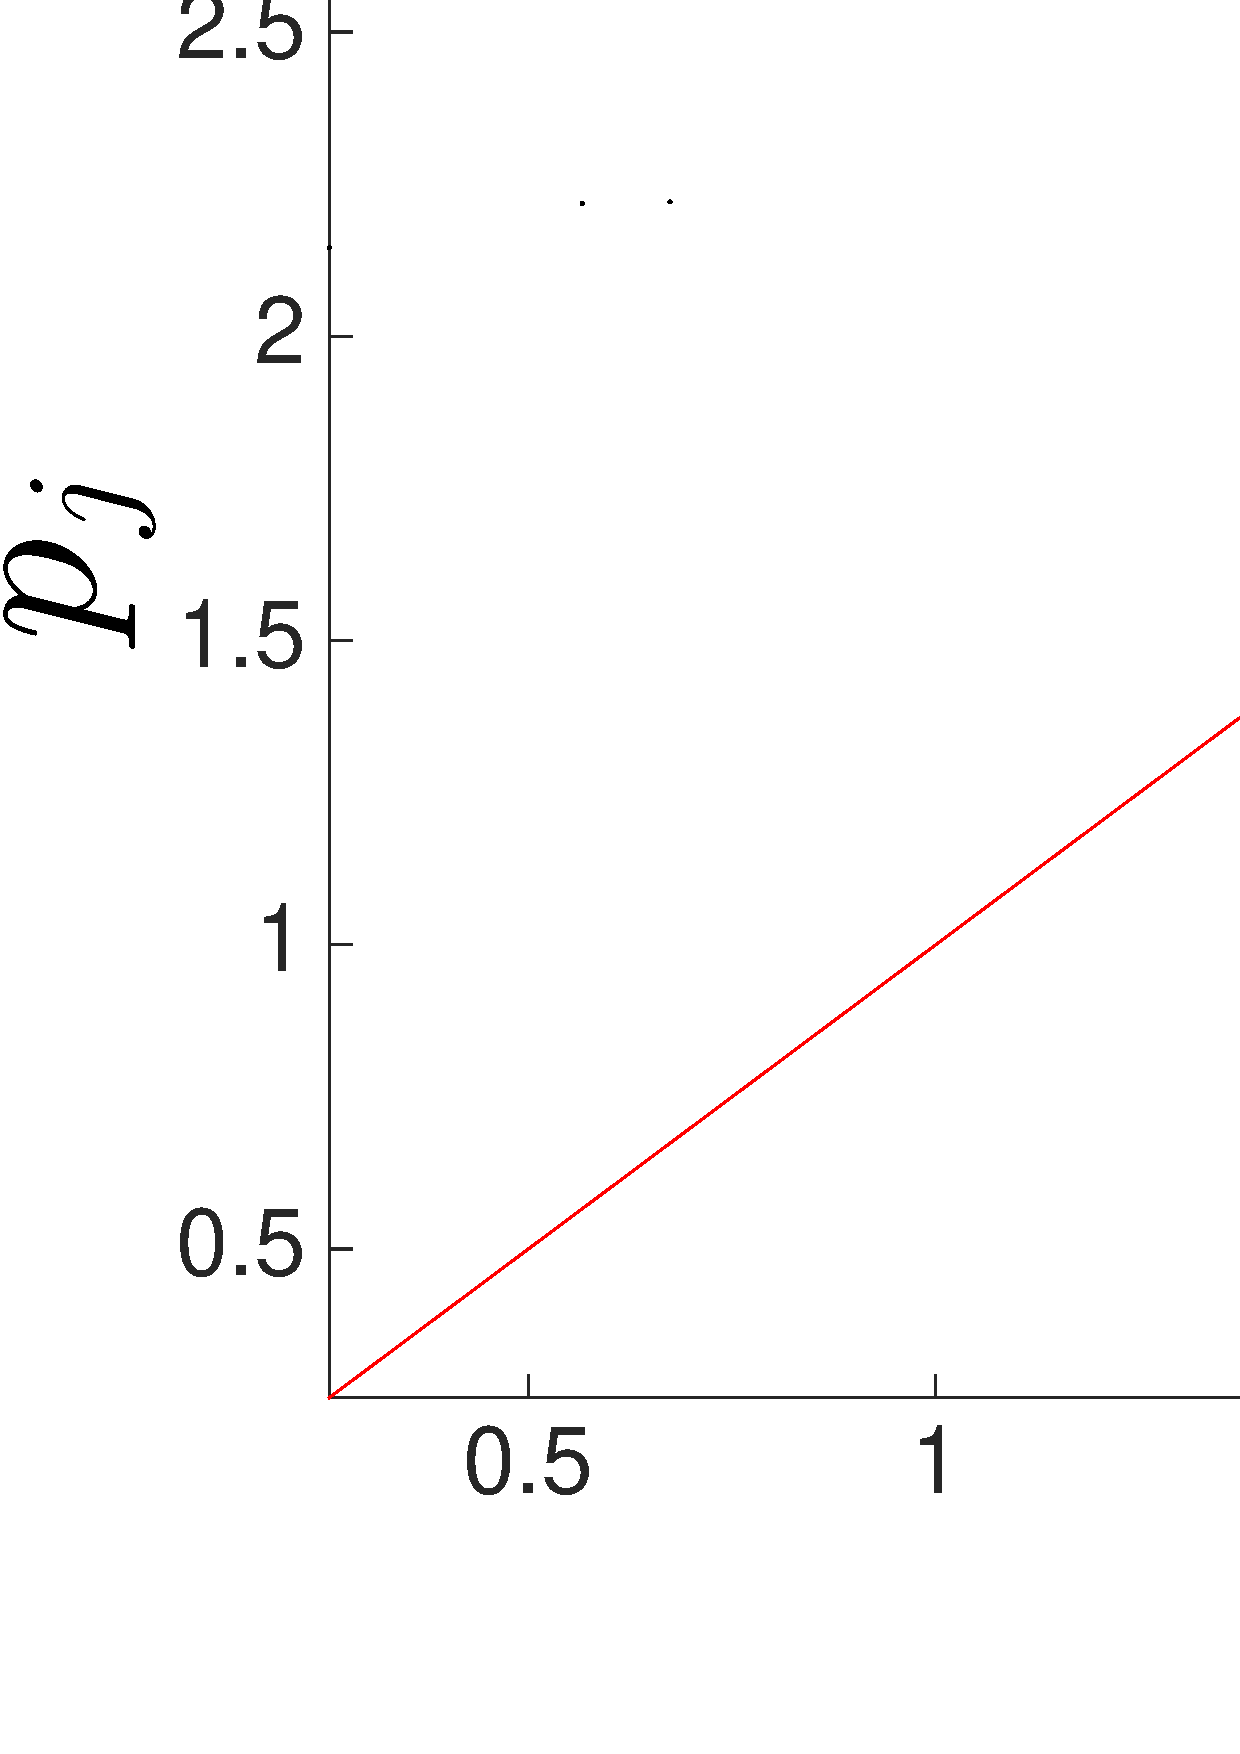
\includegraphics[width=\columnwidth]{figs/svdfiveARIMAForecast.png}
    \caption{\svdfive \\ ARIMA }
    \label{fig:gccARIMA}
  \end{subfigure}%    
  \\

      \begin{subfigure}{0.32\columnwidth}
    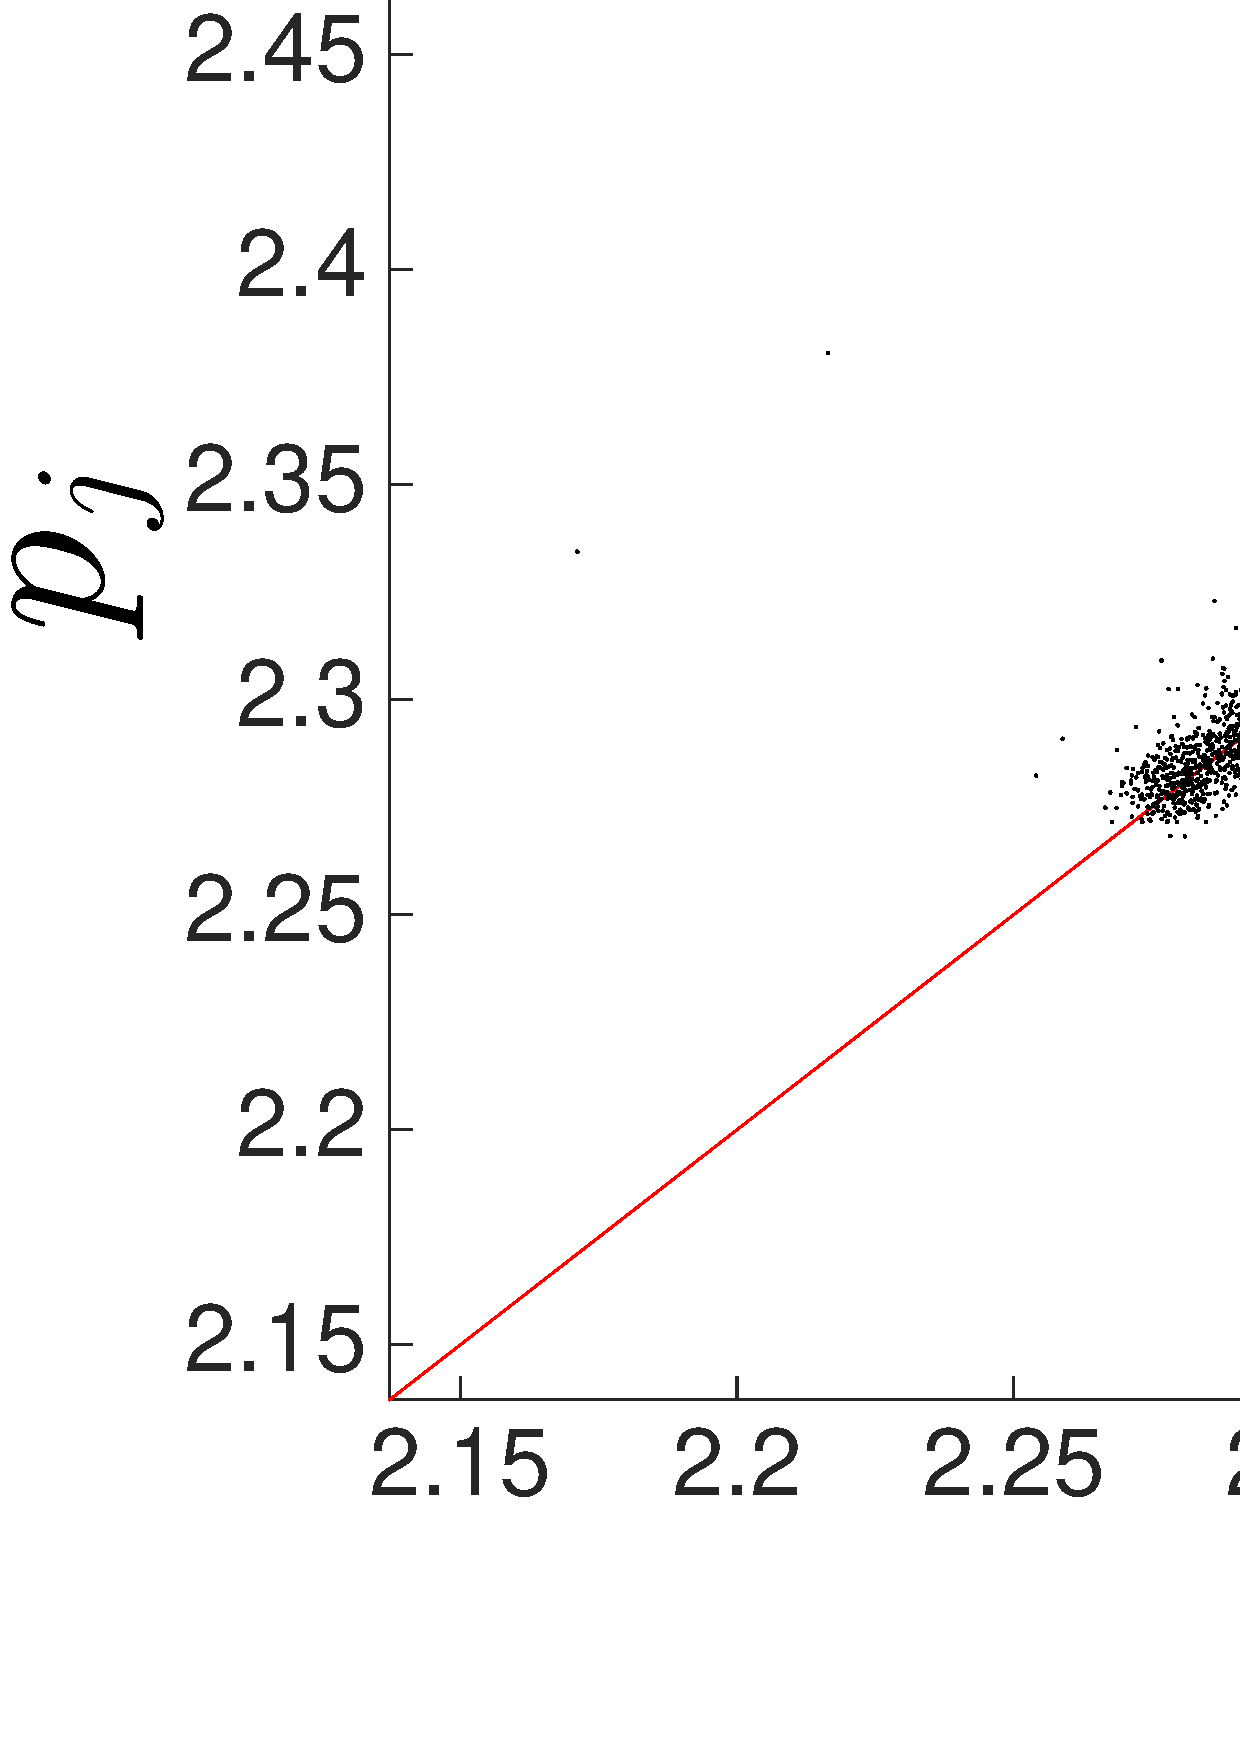
\includegraphics[width=\columnwidth]{figs/colLMAForecast.png}
    \caption{\col LMA}
    \label{fig:colLMA}
  \end{subfigure}
      \begin{subfigure}{0.32\columnwidth}
    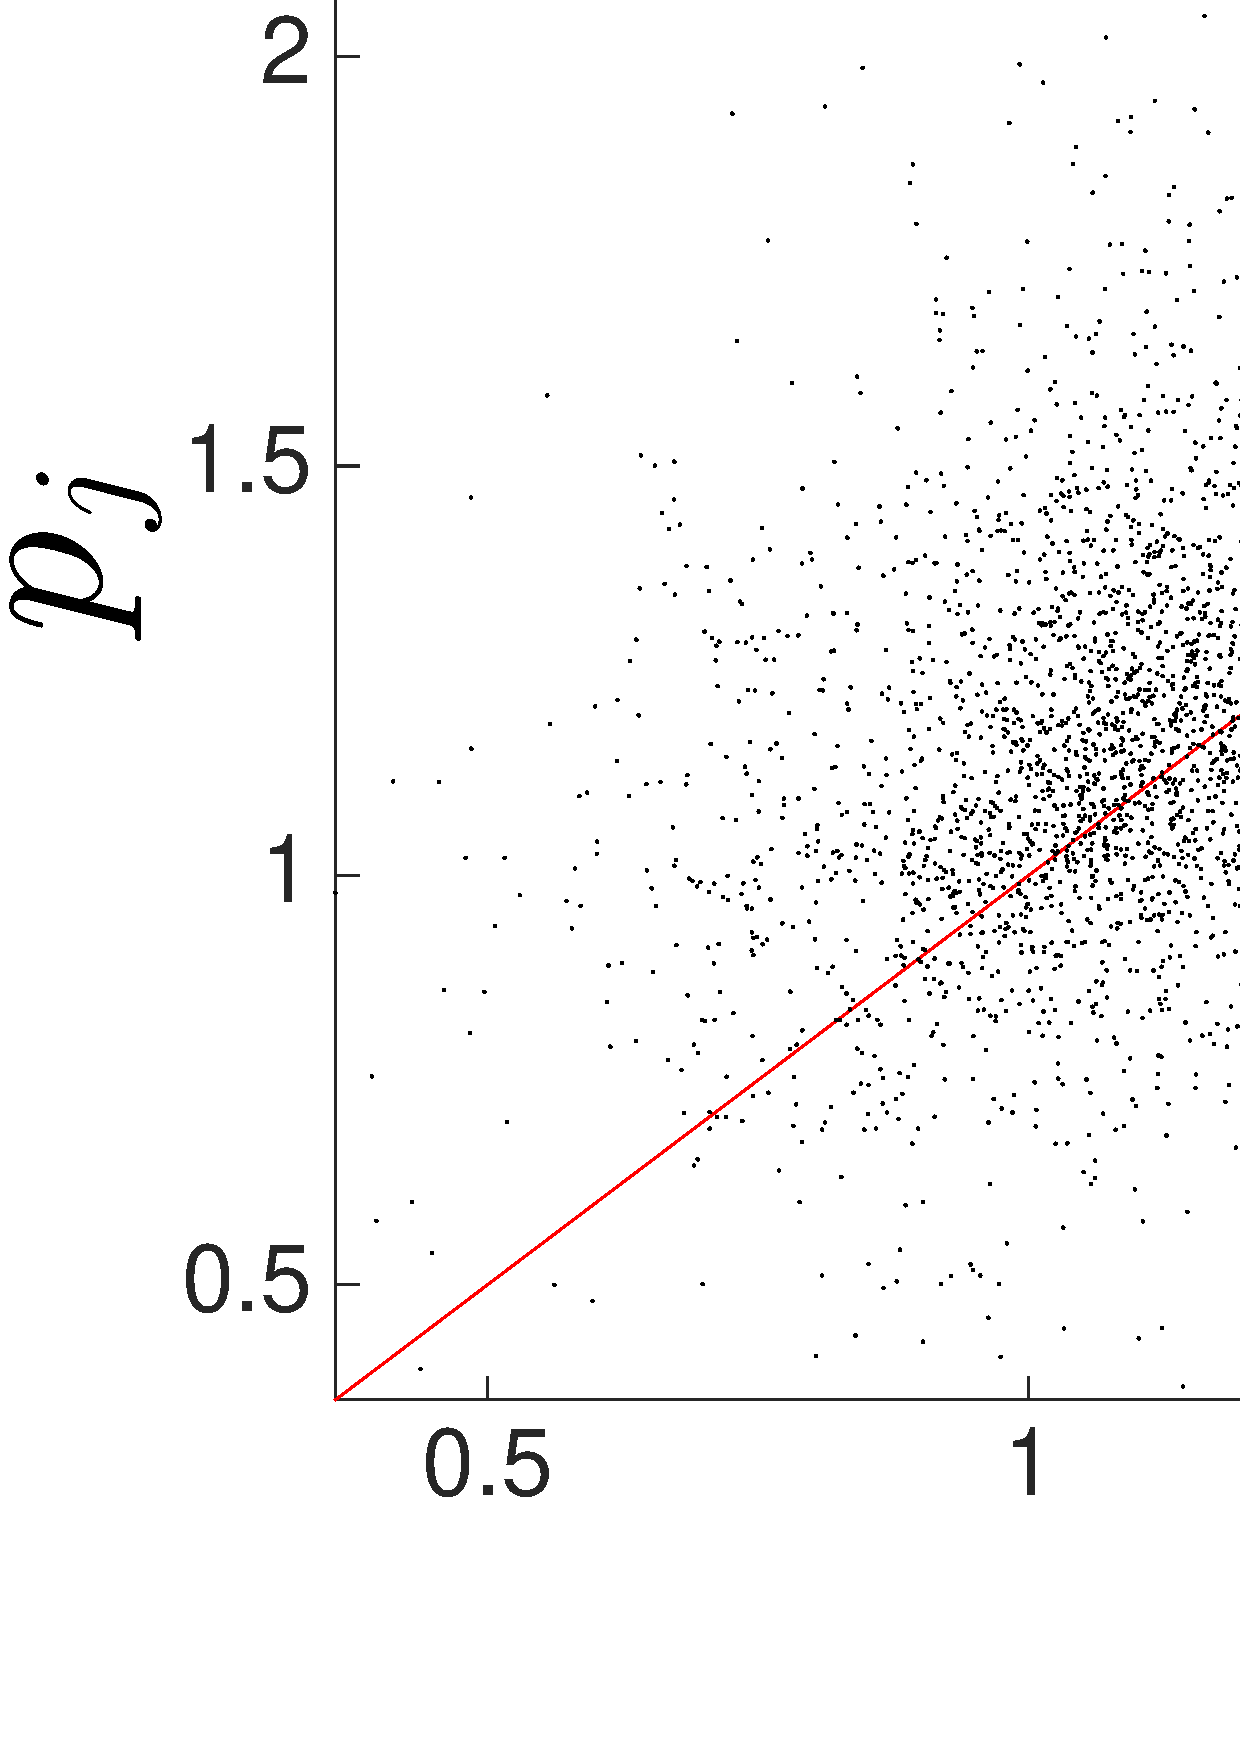
\includegraphics[width=\columnwidth]{figs/gccLMAForecast.png}
    \caption{\gcc LMA}
    \label{fig:gccLMA}
  \end{subfigure}  
        \begin{subfigure}{0.32\columnwidth}
    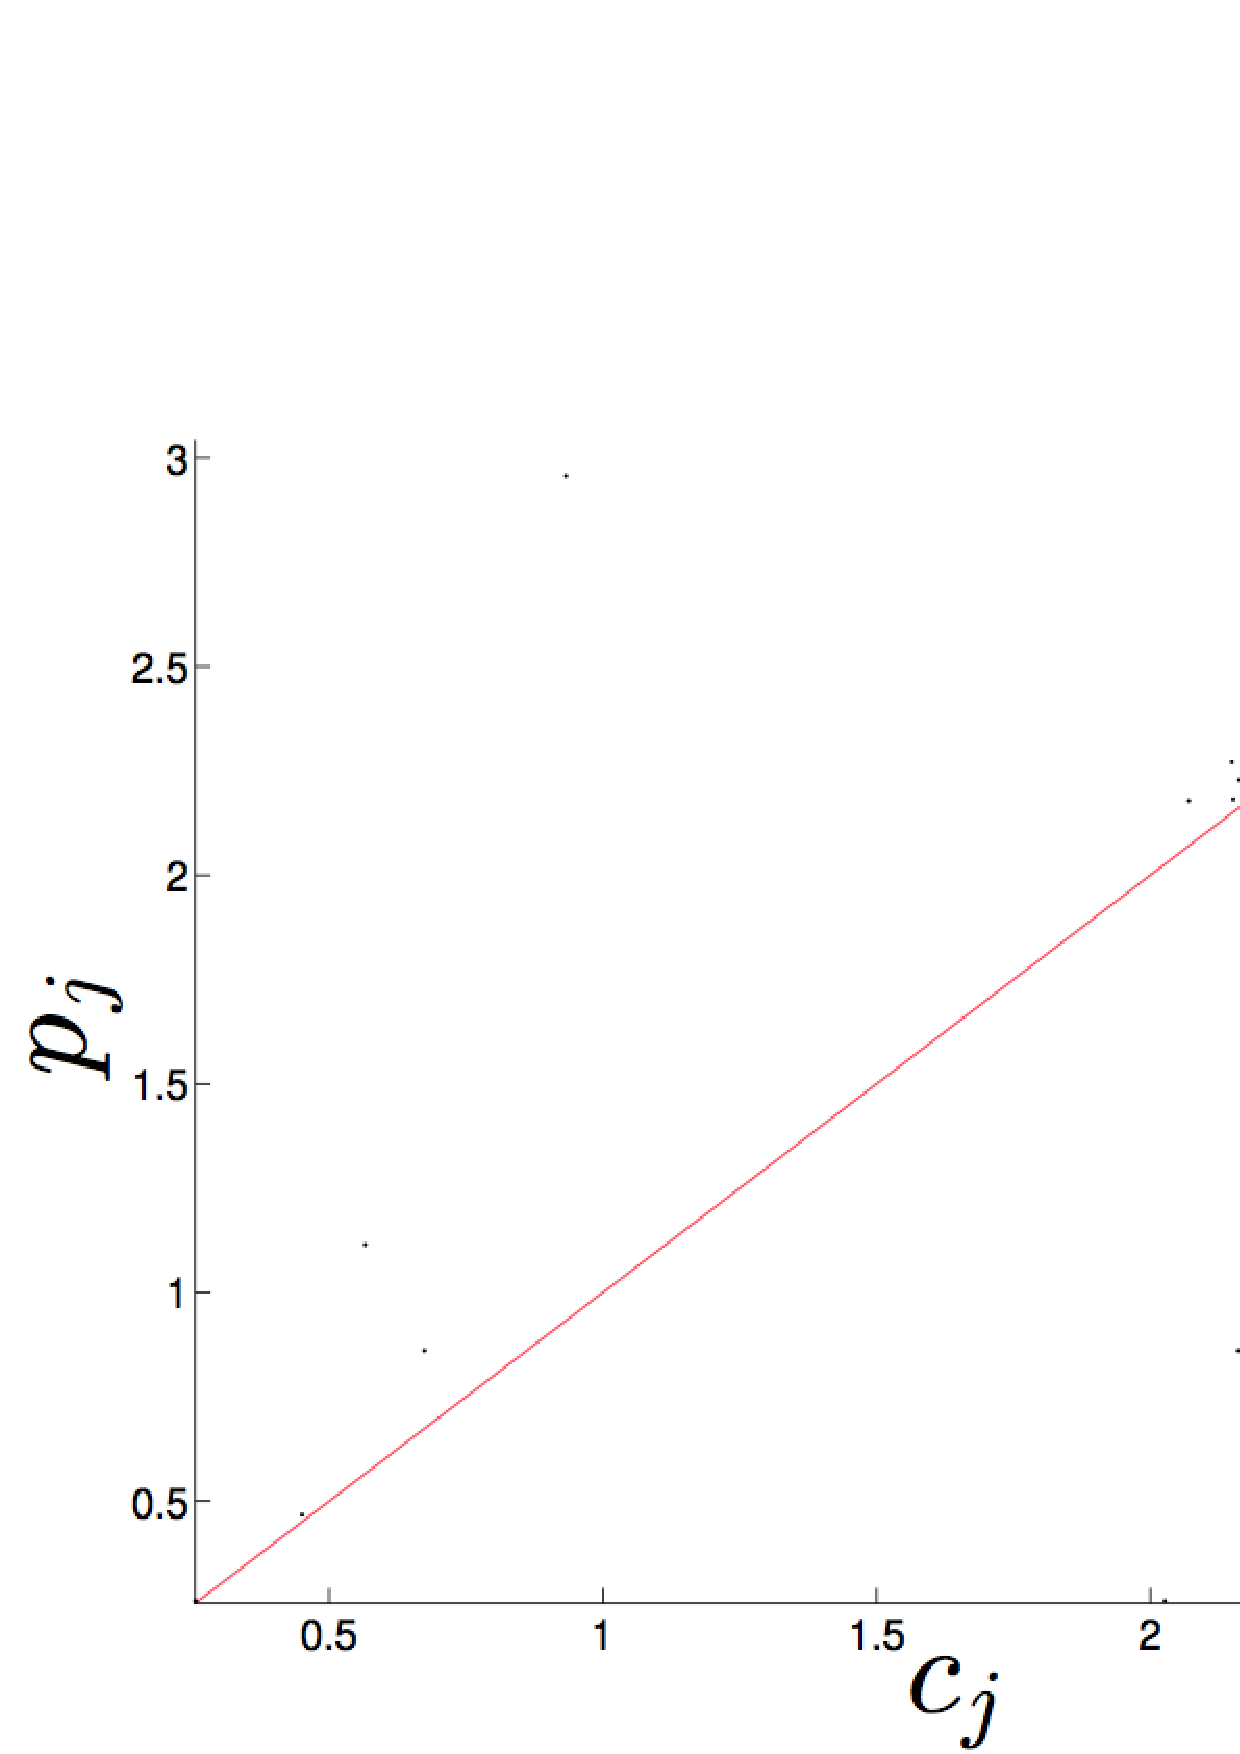
\includegraphics[width=\columnwidth]{figs/svdfiveLMAForecast.png}
    \caption{\svdfive LMA}
    \label{fig:gccLMA}
  \end{subfigure}
  %\begin{subfigure}{0.5\textwidth}
  %  \includegraphics[width=1.0\textwidth]{figs/LMA_vs_ARIMA}
   \caption{
{\color{red}[[Joshua: Liz, I added \svdfive as it has been a persistent example up to this figure. I am a little worried about the 9x9 being too small in 1 column. We may need to make this figure span two columns, which I think is ok.]]}For each of these, we plot the predicted value $p_j$ against the correct value $c_j$. On this type of plot a perfect prediction lies exactly on the diagonal, that is the line $p_j = c_j$, e.g., (g) is a near perfect prediction where-as (e) is a poor prediction.}\label{fig:forecast-example}  
  %\end{subfigure}
\end{figure} 

It may be helpful for the reader at this point to compare some of the MASE scores in Table \ref{tab:error} with the example forecasts in Figure~\ref{fig:forecast-example}. For example, if we compare Figures~ \ref{fig:forecast-example} (d) and (g), \col is almost perfectly predicted by LMA (close to the line $y=x$ and ARIMA is a poor predictor as the points are spread out around $y=x$. Comparing to the MASE values in Table~\ref{tab:error} we see that \col with LMA had a MASE of $0.05 \pm 0.002$, whereas \col with ARIMA had a MASE of $0.599 \pm 0.211$. So intuitively the better visual prediction received a much better MASE score (the smaller the better). One way of interpreting these are that LMA on \col is on average 20 times more effective than random walk and ARIMA on \col is only 2 times more effective than random walk. 

The part that becomes tricky and which must be kept in mind is that this error metric is in comparison to random walk. If we compare visually for example the LMA prediction of \col and \svdfive (Figures~\ref{fig:forecast-example} (g) \& (i)) visually they look very similar in terms of accuracy; however, \col was forecast 20 times better than random walk where as \svdfive was forecast only 1.5 times better. The reason for this lies in the strengths/weaknesses of Random Walk discussed in Section~\ref{sec:simple}. The large oscillations in \col cause Random Walk to do poorly, MASE then gives a model that accounts for this oscillation (e.g., LMA) a boost, whereas \svdfive is a great signal for Random Walk so there is less improvement to be made, and less boost is given for example for correctly reacting to regime shift. A more in-depth discussion of this is presented in Section~\ref{sec:results}. 


%[[and cherry pick a few examples of \gcc and \col to put in the text ]]


%---works quite well on the trace in Figure~%\ref{fig:ipc}, as%
%shown in Figure~\ref{fig:lmacol}. 
%
%\begin{figure}
%   \centering
%\begin{subfigure}{\columnwidth}
%    \includegraphics[width=\columnwidth]{figs/%colPredShortTS}
%    \caption{\col }
%    \label{fig:lmacol}
%  \end{subfigure}%  
%  
%    \begin{subfigure}{\columnwidth}
%    \includegraphics[width=\columnwidth]{figs/%colPredShortTS}
%    \caption{\gcc}
%    \label{fig:lmagcc}
%  \end{subfigure} 
%  \begin{subfigure}{\columnwidth}
%%    \includegraphics[width=\columnwidth]{figs/%colPredShortTS}
%    \caption{\svdfive}
%    \label{fig:lmasvdfive}
%  \end{subfigure}% 
%  \caption{{\color{red} [[If Liz thinks we should %include these I actually need to generate this %figure]]}An LMA-based forecast of
%       processor-efficiency performance trace from the%\col ,\gcc and \svdfive generating processes.  Red %circles and blue $\times$s are the true and
%       predicted values, respectively; vertical bars %show where these
%       values differ.}\label{fig:lmapredictions}
% \end{figure}
%
%\begin{figure}[htbp]
%  \centering
%   \includegraphics[width=\textwidth]{figs/colPredShortTS}
%    \caption{A forecast of the last 4,000 points of the %signal in
%      Figure~\ref{fig:ipc} using an LMA-based strategy on %the
%      embedding in Figure~\ref{fig:embedding}.  Red circles %and blue
%      $\times$s are the true and predicted values, %respectively;
%      vertical bars show where these values differ.}
%\label{fig:lmacol}
%\end{figure}
%
%\begin{figure}[htbp]
%  \centering
%    \includegraphics[width=\textwidth]{figs/colPredShortTS}
%     \caption{{\color{red} [[actually need to generate this %figure]]}An LMA-based forecast of the last 4,000 points of a
%       processor-load performance trace from the \gcc
%       benchmark.  Red circles and blue $\times$s are the %true and
%       predicted values, respectively; vertical bars show %where these
%       values differ.}
%\label{fig:lmagcc}
%\end{figure}
%
%On the other hand, if we use the same approach to %forecast the
%processor efficiency (IPC) of the \gcc time series, %the
%prediction is far less accurate; see Figure~%\ref{fig:lmagcc}.
%Figure~\ref{fig:lmasvdfive} is clearly a better %prediction than Figure~\ref{fig:gccLMA} but not nearly as good as the \col forecast.


%This gets at the utility of the contribution of this %paper: These time series all come from the same system---computers---but they are not equally predictable (at this point by LMA). For a practitioner is it the case that 
%  Our
%conjecture is that while they come from similar systems \gcc produces processor load traces on the top of the complexity spectrum whereas \col produces processor loads with complexity in the mid to low region of the complexity spectrum. If this is the case then \gcc might be much better predicted using a method like Random Walk or \naive which can effectively predict in the presence of complexity. This is explored more rigorously in the results Section of this paper (Section \ref{sec:results}. So that we don't have to compare the forecast accuarcy by visual comparing the predictions we calculate a figure of merit to compare the predictions. 





% took out for space

